%!TEX root = ../dokumentation.tex

\chapter{Stand der Technik}
Die Verwendung von Virtual Reality in der Forschung setzt sich immer weiter durch. Vor allem die Digitalisierung der Versuchsumgebung bringt einige enorme Vorteile für die Forschung mit sich. Beispielsweise können Versuche in VR beliebig oft mit genau dem gleichen Aufbau wiederholt werden. VR mit Eye-Tracking zu koppeln bietet daher sehr viele interessante Möglichkeiten\cite{Clay_Koenig_Koenig_2019}. Im Folgenden werden aktuelle Erkenntnisse zu VR in Kombination mit Eye-Tracking vorgestellt.

\section{Verwendung von Eye-Tracking in VR}
Eye-Tracking kann in Verbindung mit VR in vielen unterschiedlichen Bereichen eingesetzt werden\cite{Clay_Koenig_Koenig_2019}. Diese verschiedenen Gebiete werden in den folgenden Abschnitten näher betrachtet.
\subsection{Erforschung von Blickverhalten}
Mittels Eye-Tracking lässt sich sehr gut feststellen, worauf ein Nutzer seine Aufmerksamkeit richtet. Dies kann unter anderem in Marketing\cite{C.Wang.2019} oder anderen Gebieten eingesetzt werden, wo die wichtigsten Informationen möglichst präsent gezeigt werden sollen. 
Ein Beispiel für die Anwendung in der Forschung zum Blickverhalten ist die Forschung von \citeauthor{P.Tian.2019}, in der das Blickverhalten von Probanden in einer VR Umgebung eines brennenden Raumes analysiert wurde. Da ein brennender Raum in echt keine wiederholbaren Forschungen erlauben würde, ganz abgesehen von der Gefährdung der Probanden, bietet sich hier die Forschung mit VR an. Dadurch können Versuche mit mehreren Probanden in genau dem gleichen Umfeld mit genauen Daten durchgeführt werden. Ziel der Studie war es, eine Evaluierung der Fluchtwege in vorgefertigten Szenarios zu ermöglichen. Durch die Analyse der Blickdaten ist es möglich zu erkennen, wo der Nutzer zu welchem Zeitpunkt hinschaut. Dadurch kann festgestellt werden, ob Hinweise zum nächsten Fluchtweg schnell gefunden werden, und wenn nicht, wie Hinweise besser platziert werden können. Die Studie kam zu dem Ergebnis, dass mit dieser Methode eine bessere Evaluierung der Fluchtwege, vor allem in Gefahrensituationen möglich ist\cite{P.Tian.2019}.
Ein weiteres Beispiel zur Erforschung des Blickverhaltens bietet die Studie von \citeauthor{K.Hotta.2019}. Hier wurde das aktive Sichtfeld der Probanden untersucht, indem ein Lichtreiz im Sichtfeld des Probanden ausgelöst wird und der Proband reagiert, sobald er den Lichtreiz wahr nimmt. Das Ziel der Studie ist es, die bisherigen Forschungen, die zu diesem Thema betrieben wurden zu verbessern, indem der Versuch in VR in Verbindung mit Eye-Tracking übertragen wird. Durch die Übertragung in VR ergibt sich der Vorteil, dass der Kopf nicht mehr fixiert werden muss, da das Display mit VR am Kopf des Probanden fixiert ist. Somit sind freie Kopfbewegungen möglich, da der Bildschirm sich entsprechend mitbewegt. Desweiteren bietet der Eye-Tracker einen enormen Mehrwert, da Reaktionen der Augen direkt aufgezeichnet werden, und nicht, wie in den vorherigen Studien üblich, der Proband aktiv angeben muss, wann er den Reiz wahr nimmt. Damit war es den Forschern möglich, die Zeit pro Verscuh von rund 30 Minuten im vorherigen Versuchsaufbau auf 5 Minuten zu reduzieren und dabei verlässlichere Ergebnisse zu produzieren\cite{K.Hotta.2019}. 

\subsection{Interaktionen}


\subsection{Foveated rendering}
Der treibende Faktor hinter der Entwicklung von VR ist der Gaming Markt. Das ist daran zu erkennen, dass alle großen Firmen in der VR-Branche aus der Gaming-Branche kommen, oder über Umwege mit ihr zu tun haben. Die Geräte von HTC beispielsweise sind in Zusammenarbeit mit dem Videospiel Publisher Valve entwickelt worden, der mit SteamVR seine eigene Schnittstelle für VR Anwendungen anbietet (vgl. Abschnitt \todo{link zum SteamVR kapitel}). Valve hat mit der Valve Index mittlerweile auch ein eigenes VR-Headset auf den Markt gebracht. Der Hersteller Oculus VR, eine Tochterfirma von Facebook und einer der Pioniere der VR-Szene, hat seine erste Brille mit dem Hauptziel, VR-Gaming für die breite Masse zugänglich zu machen, auf den Markt gebracht\cite{OculusKickstarter}. Jedoch ist VR momentan noch sehr Ressourcenintensiv. Ein Blick auf die Systemanforderungen der Hersteller zeigt, dass meist ein sehr starker Computer, vor allem mit starker Grafikkarte benötigt wird, um ein angenehmes VR Erlebnis zu erzielen\cite{Lang.2019}. Die enorme Rechenkraft, die benötigt wird, um ein VR Headset zu betreiben kann allerdings reduziert werden. Hierfür wird sogenanntes Foveated Rendering genutzt. Dabei wird Eye-Tracking genutzt, um den Bereich des Bildes zu bestimmen, der vom Nutzer gerade fixiert wird (Region of Interest). Dieser Bereich wird dann in der vollen Auflösung berechnet, während der restliche Teil des Bildes in einem Bruchteil der tatsächlichen Auflösung berechnet wird. 
\begin{figure}
	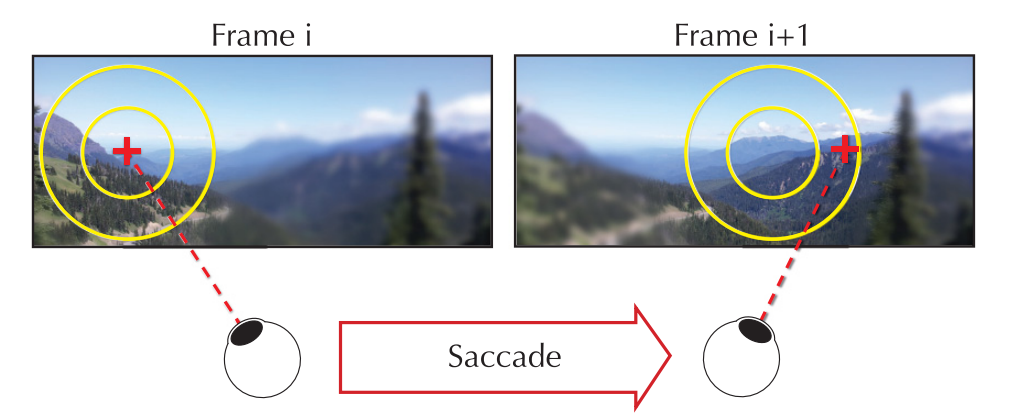
\includegraphics[width=\linewidth]{images/foveated_rendering}
	\caption{Foveated Rendering Beispiel \cite{Albert.2017}}
	\label{fig:foveated}
\end{figure}


In der Abbildung oben ist schemenhaft zu sehen, wie Foveated Rendering funktioniert. Der Bereich, der fokussiert wird, wird scharf dargestellt. Der Bereich rund um den fokussierten Bereich wird ebenfalls scharf dargestellt, allerdings nicht so scharf wie der Hauptbereich.  Der restliche Bereich wird unscharf dargestellt. Da der Nutzer diesen Bereich nicht aktiv anschaut, fällt auch die geringere Auflösung nicht auf. Während einer Sakkade werden Objekte vom Auge nicht komplett scharf wahrgenommen, weshalb es für den Nutzer nicht spürbar ist, dass ein Bereich des Bildes nicht scharf dargestellt wird. Die Zeit, bis das Auge sich auf einen neuen Punkt fixiert hat ist ausreichend, um das Bild in diesem Bereich scharf zu stellen, so dass dem Nutzer der Einsatz von Foveated Rendering nicht auffällt\cite{Albert.2017}. Der Einsatz von Foveated Rendering kann die Last auf den Computer deutlich reduzieren. In ersten Versuchen ist eine Erhöhung der Bilder pro Sekunde (Frames per Second, fps) von 10-15 Prozent beobachtbar gewesen\cite{H.Kim.2018}.

\section{Steuermöglichkeiten in VR}
\subsection{Herkömmliche Steuerarten}
Unterteilung in zwei Gruppen:
- Standard PC Inupt devices wie tastatur, maus, controller
- VR spezifische input devices -> Vive Controller
\subsection{Hand-Tracking}
Leap Motion
\subsection{Eye-Tracking und Head-Tracking}
Electrooculogramm, Kamerabasiert
head gaze https://ieeexplore.ieee.org/document/7519387
data gloves https://ieeexplore.ieee.org/document/7988640
electrooculogram https://ieeexplore.ieee.org/document/7732407
eye tracking mit arm zucken https://link.springer.com/article/10.1007/s10055-018-0371-2
\section{Bisherige Erkenntnisse zu Eye-Tracking als Steuerung im Vergleich zu anderen Steuermöglichkeiten}

\section{Interaction techniques using head gaze for virtual reality}

\label{paper1}
Diese im Mai 2016 veröffentlichte Arbeit hat sich zum Ziel gesetzt, die Position des Kopfes zu nutzen, um die ungefähre Blickrichtung des Nutzers zu erkennen und somit natürlichere Interaktionen in der virtuellen Realität zu ermöglichen. Die Motivation hinter der Arbeit war es, die doch sehr unnatürliche Steuerung über Controller zu ersetzen, um so eine bessere Immersion in die virtuelle Welt zu gewährleisten. Die Wahl, die Kopfbewegung als Steuerung zu nutzen, ist gefallen, da diese Bewegung von allen natürlcih vorkommenden interaktiven Bewegungen eines Nutzers (wie z.B. Handbewegungen, Augenbewegungen, Fuß/Beinbewegungen und Kopfbewegungen) am einfachsten zu erfassen und in VR übertragbar ist. Da ein Großteil der VR-Headsets auf dem Erfassen des Kopfes in einem Raum basiert (TODO vgl Kpaitel von Jörn wie er des erklärt), ist die Erfassung dieser Daten meist ohne größere Umstände möglich. Um ein Aussagekräftiges Ergebnis zu erlangen, wurden mehrere Versuchsreihen und anschließende Befragungen der Probanden durchgeführt. Die Autoren der Arbeit haben dafür einige Spiele (teils bereits in VR existierend, teils Portierungen von Smartphone Spielen in VR) so angepasst, dass Kopfbewegungen zur Steuerung eingelesen werden können. Als Eingabegeräte wurden ein Leap Motion Controller (ein Hand-Tracking Gerät), ein herkömmlicher XBox Controller und das von den Autoren "Head Gaze" benannte Kopf-Tracking miteinander verglichen. Als VR-Headset wurde ein Oculus DK2 verwendet. 
Nach der ersten Versuchsreihe in dem Spiel "Slash the Fruit VR" hat sich Head Gaze als die intuitivste Eingabemethode herausgestellt. Daher wurden in den nachfolgenden beiden Versuchen mit den Spielen "Virtual Reality Experience" (kurz VREx) und "Dungeon VR" nur noch Head Gaze verwendet. Der Grund hierfür war zum Einen die Unzuverlässigkeit des Leap Motion Controllers, zum Anderen war der XBox Controller nicht intuitiv genug für Bewegungen in VR. 
Da die Kernfrage die Immersion der neuen Steuerung war, wurden die Teilnehmer der Versuchsreihe nach ihrem Immersionsbefindnis befragt.

\begin{figure}
	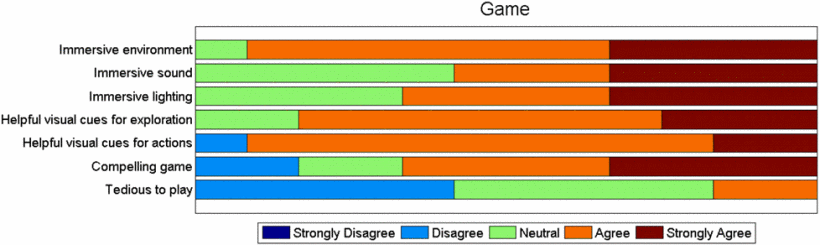
\includegraphics[width=\linewidth]{images/study1immersion}
	\caption{Resultat der Befragung}
	\label{fig:result1}
\end{figure}

Wie in den oben stehenden Ergebnissen zu sehen ist, empfand der Großteil der Nutzer diese Steuerung als immersiv und nur wenige Nutzer haben sich von der Steuerung gestört gefühlt. Als weiteres Ziel der Forscher wird von den Forschern eine Umsetzung in Smartphone VR-Anwendungen erwähnt.
\subsection{Einordnung der Relevanz}
Die beschriebene Arbeit ist für den in dieser Arbeit vorgesehenen Versuchsaufbau von großer Relevanz, da es zu einem gewissen Grad eine Vorstufe darstellt. Der Begriff Head Gaze wird von den Forschern bewusst verwendet, da mit der Kopfbewegung auch der Blick (engl. Gaze) angenommen werden kann. Somit sind der Versuchsaufbau und die damit einhergehenden Ergebnisse sehr gut mit den in dieser Arbeit entstandenen Ergebnissen vergleichbar. (TODO Vergleich) 

\section{Electrooculogram-based virtual reality game control using blink detection and gaze calibration}
Diese im September 2016 vorgestellte Arbeit beschreibt die Verwendung von einem Elektrookulogramm zur Bestimmung der Blickrichtung und zum Erkennen von Blinzeln. Diese Daten werden dann als Eingabe in einem VR-Spiel verwendet. 
Ein Elektrookulogramm (EOG) ist die Registrierung von Bewegungen der Muskeln, die zur Kontrolle der Augen dienen. Dabei werden an jeder Seite der Augenhöhle außerhalb Elektroden angebracht, mit welchen die Bewegung der Augen und Augenlider aufgezeichnet werden kann. 
Wie schon in Kapitel~\ref{paper1}, lag auch hier das Ziel dabei, eine intuitivere und immersivere Eingabemethode zu entwickeln. Zur Überprüfung der Ergebnisse werden sowohl die Rate der falschen Eingaben als auch die subjektive Empfindung erfasst. Als Beispielapplikation wird das Spiel "VRrailSurfer" verwendet. Das Spielprinzip ist vergleichbar mit dem bekannten Smartphone Spiel "Subway Surfers" Eine Bewegung der Augen nach links oder rechts hat eine Bewegung der Spielfigur in die entsprechende Richtung zur Folge. Zum Springen müssen die Augen nach oben bewegt werden. Die mit dieser Methode erzielte Genauigkeit der Steuerung lag nach einer Reihe von Versuchen mit 10 Probanden im Durchschnitt bei 78\%, wohingegen die Blinzelerkennung mit 96\% deutlich höher lag. Die Forscher haben allerdings in diesem Beispiel nur die Steuerung über den Blick im Spiel implementiert, sie gehen aber davon aus, dass eine Genauigkeit von rund 96\% auch in einem Spiel mit Blinzelerkennung umsetzbar ist. 
\subsection{Einordnung der Relevanz}
Das Paper ist für diese Arbeit auch relevant. Trotz der komplett anderen Eye-Tracking Methode sind einige Punkte auf diese Arbeit übertragbar. Der Ansatz, Augenbewegungen über ein EOG zu erfassen, ist allerdings eher suboptimal, da die Genauigkeit nicht so hoch ist, wie bei dem in dieser Arbeit verwendeten System, da mehr Komplikationen, wie etwa ein verrutschen der Elektroden, auftreten können. Der Fokus des Papers lag allerdings eher auf der Machbarkeit eines EOGs in Verbindung mit einem VR-Headset, weshalb kein Vergleich mit anderen Eingabemethoden stattgefunden hat. 




